\documentclass[10pt]{article}

\usepackage{amsfonts,latexsym,amsthm,amssymb,amsmath,amscd,euscript}
\def\arraystretch{1.2}

\usepackage{bold-extra}
\usepackage{framed}
\usepackage{minted}
\usepackage{graphicx}
\usepackage[geometry]{ifsym}
\usepackage{hyperref}
\hypersetup{colorlinks=true,citecolor=blue,urlcolor=blue,linkbordercolor={1 0 0}}

\textwidth=14.5cm \textheight=20.0cm
\oddsidemargin=1cm
\evensidemargin=1cm

\title{CS181 Practical 4: Swingy Monkey!} 
\author{Victor Domene, Henrique Vaz, Joshua Meier} 
\date{April 28th, 2016}

\begin{document}

\maketitle

\section{Abstract} 

In this practical, we performed machine learning on Swingy Monkey, a game
based on the viral game Flappy Bird that took off a few years ago.
In Swingy Monkey, at any point in time, there are only two possible actions:
to jump, or not to jump. 

In this practical, we performed machine learning on
truncated lists of user / artist play counts, in order to predict how many
times each of these users listened to every artist in the collection. The
implications of high accuracy here are quite interesting - there are many
commercial applications to being able to predict a user's entire play history
from just a few sample points. However, this also makes the problem extremely
difficult. Unlike previous practicals where we had complete training data to
work with, we did not necessarily have complete data for each user in the
training set, and furthermore, we did not have a completeness metric for the
data of any user. After performing a thorough data analysis to better
understand the complexity of the data, we then continued to apply a variety of
very different machine learning techniques, since many different intuitions
could be applied here. We also performed feature engineering, but we were
unable to incorporate these features (known as "side information" in the
literature) into the algorithms in a fashion that allowed the algorithms to
terminate in reasonable time. Ultimately, we discovered that a simple matrix
factorization using just a single feature performed best, giving us the fourth
position in the Public Leaderboard (as of 2pm on Friday). Notably, our
hand-crafted matrix factorization algorithm outperformed several
implementations from popular software packages. 

\section{Technical Approach} 

\subsection{Dependencies}

\subsection{Data Analysis and Centering} 

%\begin{center} 
%\begin{tabular}{c c} 
%\hline 
%\hline
%mean & $4506.2$ \\ \hline
%median &  $2639$ \\ \hline 
%standard deviation & $6467.843$ \\ \hline 
%max & $453683$ \\ \hline 
%min & $9$ \\ \hline 
%\hline 
%\end{tabular} 
%\end{center}

%\begin{figure}[h] 
%\centering
%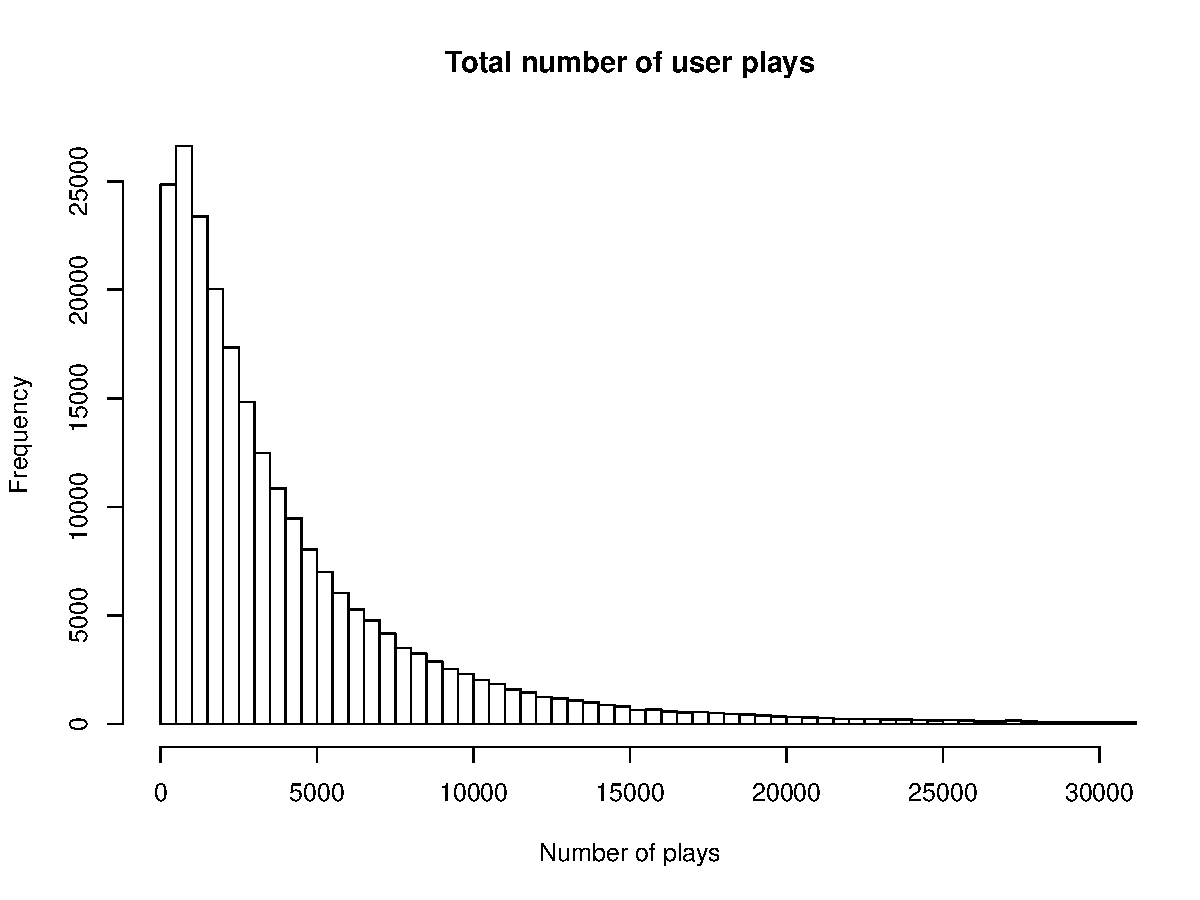
\includegraphics[width=0.8\textwidth]{../experiments/total_counts.pdf}
%\caption{Histogram of the total number of user plays from the train data. This
%plot is right truncated since there are several users (but not many) with large
%number of plays. Including all this information would make it difficult to
%observe the half-normal distribution of the data. In particular, note that
%there is a user with $453683$ total plays.} 
%\label{fig:img3} 
%\end{figure}

\subsection{Feature Engineering: Handling the State Space} 

\subsubsection{Choosing the Features}

\subsubsection{Binning}

\subsection{Q-Learning}

\subsubsection{$\epsilon$-greedy}

\subsection{Parameter Tuning}

\subsubsection{Learning Rate: $\alpha$}

\subsubsection{Discount Rate: $\gamma$}

\subsubsection{Randomness: $\epsilon$}

\subsubsection{Number of Bins}

\subsection{Supervised Approach: For Fun!}

\section{Code}

Our code for this practical can be found in this
\href{https://github.com/victordomene/cs181-practicals/tree/master/practical4}{GitHub
Repository}. There is a README file with some setup instructions.

\end{document}
